
%% bare_jrnl_compsoc.tex
%% V1.3
%% 2007/01/11
%% by Michael Shell
%% See:
%% http://www.michaelshell.org/
%% for current contact information.
%%
%% This is a skeleton file demonstrating the use of IEEEtran.cls
%% (requires IEEEtran.cls version 1.7 or later) with an IEEE Computer
%% Society journal paper.
%%
%% Support sites:
%% http://www.michaelshell.org/tex/ieeetran/
%% http://www.ctan.org/tex-archive/macros/latex/contrib/IEEEtran/
%% and
%% http://www.ieee.org/

%%*************************************************************************
%% Legal Notice:
%% This code is offered as-is without any warranty either expressed or
%% implied; without even the implied warranty of MERCHANTABILITY or
%% FITNESS FOR A PARTICULAR PURPOSE! 
%% User assumes all risk.
%% In no event shall IEEE or any contributor to this code be liable for
%% any damages or losses, including, but not limited to, incidental,
%% consequential, or any other damages, resulting from the use or misuse
%% of any information contained here.
%%
%% All comments are the opinions of their respective authors and are not
%% necessarily endorsed by the IEEE.
%%
%% This work is distributed under the LaTeX Project Public License (LPPL)
%% ( http://www.latex-project.org/ ) version 1.3, and may be freely used,
%% distributed and modified. A copy of the LPPL, version 1.3, is included
%% in the base LaTeX documentation of all distributions of LaTeX released
%% 2003/12/01 or later.
%% Retain all contribution notices and credits.
%% ** Modified files should be clearly indicated as such, including  **
%% ** renaming them and changing author support contact information. **
%%
%% File list of work: IEEEtran.cls, IEEEtran_HOWTO.pdf, bare_adv.tex,
%%                    bare_conf.tex, bare_jrnl.tex, bare_jrnl_compsoc.tex
%%*************************************************************************

% *** Authors should verify (and, if needed, correct) their LaTeX system  ***
% *** with the testflow diagnostic prior to trusting their LaTeX platform ***
% *** with production work. IEEE's font choices can trigger bugs that do  ***
% *** not appear when using other class files.                            ***
% The testflow support page is at:
% http://www.michaelshell.org/tex/testflow/

% Note that the a4paper option is mainly intended so that authors in
% countries using A4 can easily print to A4 and see how their papers will
% look in print - the typesetting of the document will not typically be
% affected with changes in paper size (but the bottom and side margins will).
% Use the testflow package mentioned above to verify correct handling of
% both paper sizes by the user's LaTeX system.
%
% Also note that the "draftcls" or "draftclsnofoot", not "draft", option
% should be used if it is desired that the figures are to be displayed in
% draft mode.
%
% The Computer Society usually requires 10pt for submissions.
%
\documentclass[conference]{IEEEtran}
%
% If IEEEtran.cls has not been installed into the LaTeX system files,
% manually specify the path to it like:
% \documentclass[12pt,journal,compsoc]{../sty/IEEEtran}

% Some very useful LaTeX packages include:
% (uncomment the ones you want to load)

% *** MISC UTILITY PACKAGES ***
%
%\usepackage{ifpdf}
% Heiko Oberdiek's ifpdf.sty is very useful if you need conditional
% compilation based on whether the output is pdf or dvi.
% usage:
% \ifpdf
%   % pdf code
% \else
%   % dvi code
% \fi
% The latest version of ifpdf.sty can be obtained from:
% http://www.ctan.org/tex-archive/macros/latex/contrib/oberdiek/
% Also, note that IEEEtran.cls V1.7 and later provides a builtin
% \ifCLASSINFOpdf conditional that works the same way.
% When switching from latex to pdflatex and vice-versa, the compiler may
% have to be run twice to clear warning/error messages.

\usepackage{listings}
\usepackage{color}

\definecolor{codegreen}{rgb}{0,0.6,0}
\definecolor{codegray}{rgb}{0.5,0.5,0.5}
\definecolor{codepurple}{rgb}{0.58,0,0.82}
\definecolor{backcolour}{rgb}{0.95,0.95,0.92}
 
\lstdefinestyle{mystyle}{
    language=Python,
    backgroundcolor=\color{backcolour},   
    commentstyle=\color{codegreen},
    keywordstyle=\color{magenta},
    numberstyle=\tiny\color{codegray},
    stringstyle=\color{codepurple},
    basicstyle=\footnotesize,% basic font setting
    breakatwhitespace=false,         
    breaklines=true,                 
    captionpos=b,                    
    keepspaces=true,                 
    numbers=left,                    
    numbersep=5pt,                  
    showspaces=false,                
    showstringspaces=false,
    showtabs=false,                  
    tabsize=2
}
\lstset{style=mystyle}

\usepackage{url}
\usepackage{alltt}
\usepackage{epsfig}
%\usepackage{multirow}
%\usepackage{multicol}
%\usepackage{alltt}
\usepackage{times}
\usepackage{fancyhdr}
\usepackage{graphicx}
\usepackage{amsmath}

\newcommand{\ignore}[1]{}

\newcommand{\totallinewritesbeforesystemfailure}{\mathtt{Total\ Line\ Writes\ Before\ System\ Failure}}
\newcommand{\totallinewritesbeforesystemfailurewithecp}{\mathtt{Total\ Line\ Writes\ Before\ System\ Failure\ With\ Uniform\ ECP6 }}

% *** CITATION PACKAGES ***
%
\ifCLASSOPTIONcompsoc
  % IEEE Computer Society needs nocompress option
  % requires cite.sty v4.0 or later (November 2003)
  % \usepackage[nocompress]{cite}
\else
  % normal IEEE
  % \usepackage{cite}
\fi
% cite.sty was written by Donald Arseneau
% V1.6 and later of IEEEtran pre-defines the format of the cite.sty package
% \cite{} output to follow that of IEEE. Loading the cite package will
% result in citation numbers being automatically sorted and properly
% "compressed/ranged". e.g., [1], [9], [2], [7], [5], [6] without using
% cite.sty will become [1], [2], [5]--[7], [9] using cite.sty. cite.sty's
% \cite will automatically add leading space, if needed. Use cite.sty's
% noadjust option (cite.sty V3.8 and later) if you want to turn this off.
% cite.sty is already installed on most LaTeX systems. Be sure and use
% version 4.0 (2003-05-27) and later if using hyperref.sty. cite.sty does
% not currently provide for hyperlinked citations.
% The latest version can be obtained at:
% http://www.ctan.org/tex-archive/macros/latex/contrib/cite/
% The documentation is contained in the cite.sty file itself.
%
% Note that some packages require special options to format as the Computer
% Society requires. In particular, Computer Society  papers do not use
% compressed citation ranges as is done in typical IEEE papers
% (e.g., [1]-[4]). Instead, they list every citation separately in order
% (e.g., [1], [2], [3], [4]). To get the latter we need to load the cite
% package with the nocompress option which is supported by cite.sty v4.0
% and later. Note also the use of a CLASSOPTION conditional provided by
% IEEEtran.cls V1.7 and later.

% *** GRAPHICS RELATED PACKAGES ***
%
\ifCLASSINFOpdf
  % \usepackage[pdftex]{graphicx}
  % declare the path(s) where your graphic files are
  % \graphicspath{{../pdf/}{../jpeg/}}
  % and their extensions so you won't have to specify these with
  % every instance of \includegraphics
  % \DeclareGraphicsExtensions{.pdf,.jpeg,.png}
\else
  % or other class option (dvipsone, dvipdf, if not using dvips). graphicx
  % will default to the driver specified in the system graphics.cfg if no
  % driver is specified.
  % \usepackage[dvips]{graphicx}
  % declare the path(s) where your graphic files are
  % \graphicspath{{../eps/}}
  % and their extensions so you won't have to specify these with
  % every instance of \includegraphics
  % \DeclareGraphicsExtensions{.eps}
\fi
% graphicx was written by David Carlisle and Sebastian Rahtz. It is
% required if you want graphics, photos, etc. graphicx.sty is already
% installed on most LaTeX systems. The latest version and documentation can
% be obtained at: 
% http://www.ctan.org/tex-archive/macros/latex/required/graphics/
% Another good source of documentation is "Using Imported Graphics in
% LaTeX2e" by Keith Reckdahl which can be found as epslatex.ps or
% epslatex.pdf at: http://www.ctan.org/tex-archive/info/
%
% latex, and pdflatex in dvi mode, support graphics in encapsulated
% postscript (.eps) format. pdflatex in pdf mode supports graphics
% in .pdf, .jpeg, .png and .mps (metapost) formats. Users should ensure
% that all non-photo figures use a vector format (.eps, .pdf, .mps) and
% not a bitmapped formats (.jpeg, .png). IEEE frowns on bitmapped formats
% which can result in "jaggedy"/blurry rendering of lines and letters as
% well as large increases in file sizes.
%
% You can find documentation about the pdfTeX application at:
% http://www.tug.org/applications/pdftex

% *** MATH PACKAGES ***
%
%\usepackage[cmex10]{amsmath}
% A popular package from the American Mathematical Society that provides
% many useful and powerful commands for dealing with mathematics. If using
% it, be sure to load this package with the cmex10 option to ensure that
% only type 1 fonts will utilized at all point sizes. Without this option,
% it is possible that some math symbols, particularly those within
% footnotes, will be rendered in bitmap form which will result in a
% document that can not be IEEE Xplore compliant!
%
% Also, note that the amsmath package sets \interdisplaylinepenalty to 10000
% thus preventing page breaks from occurring within multiline equations. Use:
%\interdisplaylinepenalty=2500
% after loading amsmath to restore such page breaks as IEEEtran.cls normally
% does. amsmath.sty is already installed on most LaTeX systems. The latest
% version and documentation can be obtained at:
% http://www.ctan.org/tex-archive/macros/latex/required/amslatex/math/

% *** SPECIALIZED LIST PACKAGES ***
%
%\usepackage{algorithmic}
% algorithmic.sty was written by Peter Williams and Rogerio Brito.
% This package provides an algorithmic environment fo describing algorithms.
% You can use the algorithmic environment in-text or within a figure
% environment to provide for a floating algorithm. Do NOT use the algorithm
% floating environment provided by algorithm.sty (by the same authors) or
% algorithm2e.sty (by Christophe Fiorio) as IEEE does not use dedicated
% algorithm float types and packages that provide these will not provide
% correct IEEE style captions. The latest version and documentation of
% algorithmic.sty can be obtained at:
% http://www.ctan.org/tex-archive/macros/latex/contrib/algorithms/
% There is also a support site at:
% http://algorithms.berlios.de/index.html
% Also of interest may be the (relatively newer and more customizable)
% algorithmicx.sty package by Szasz Janos:
% http://www.ctan.org/tex-archive/macros/latex/contrib/algorithmicx/

% *** ALIGNMENT PACKAGES ***
%
%\usepackage{array}
% Frank Mittelbach's and David Carlisle's array.sty patches and improves
% the standard LaTeX2e array and tabular environments to provide better
% appearance and additional user controls. As the default LaTeX2e table
% generation code is lacking to the point of almost being broken with
% respect to the quality of the end results, all users are strongly
% advised to use an enhanced (at the very least that provided by array.sty)
% set of table tools. array.sty is already installed on most systems. The
% latest version and documentation can be obtained at:
% http://www.ctan.org/tex-archive/macros/latex/required/tools/

%\usepackage{mdwmath}
%\usepackage{mdwtab}
% Also highly recommended is Mark Wooding's extremely powerful MDW tools,
% especially mdwmath.sty and mdwtab.sty which are used to format equations
% and tables, respectively. The MDWtools set is already installed on most
% LaTeX systems. The lastest version and documentation is available at:
% http://www.ctan.org/tex-archive/macros/latex/contrib/mdwtools/

% IEEEtran contains the IEEEeqnarray family of commands that can be used to
% generate multiline equations as well as matrices, tables, etc., of high
% quality.

%\usepackage{eqparbox}
% Also of notable interest is Scott Pakin's eqparbox package for creating
% (automatically sized) equal width boxes - aka "natural width parboxes".
% Available at:
% http://www.ctan.org/tex-archive/macros/latex/contrib/eqparbox/

% *** SUBFIGURE PACKAGES ***
%\ifCLASSOPTIONcompsoc
%\usepackage[tight,normalsize,sf,SF]{subfigure}
%\else
%\usepackage[tight,footnotesize]{subfigure}
%\fi
% subfigure.sty was written by Steven Douglas Cochran. This package makes it
% easy to put subfigures in your figures. e.g., "Figure 1a and 1b". For IEEE
% work, it is a good idea to load it with the tight package option to reduce
% the amount of white space around the subfigures. Computer Society papers
% use a larger font and \sffamily font for their captions, hence the
% additional options needed under compsoc mode. subfigure.sty is already
% installed on most LaTeX systems. The latest version and documentation can
% be obtained at:
% http://www.ctan.org/tex-archive/obsolete/macros/latex/contrib/subfigure/
% subfigure.sty has been superceeded by subfig.sty.

%\ifCLASSOPTIONcompsoc
%  \usepackage[caption=false]{caption}
%  \usepackage[font=normalsize,labelfont=sf,textfont=sf]{subfig}
%\else
%  \usepackage[caption=false]{caption}
%  \usepackage[font=footnotesize]{subfig}
%\fi
% subfig.sty, also written by Steven Douglas Cochran, is the modern
% replacement for subfigure.sty. However, subfig.sty requires and
% automatically loads Axel Sommerfeldt's caption.sty which will override
% IEEEtran.cls handling of captions and this will result in nonIEEE style
% figure/table captions. To prevent this problem, be sure and preload
% caption.sty with its "caption=false" package option. This is will preserve
% IEEEtran.cls handing of captions. Version 1.3 (2005/06/28) and later 
% (recommended due to many improvements over 1.2) of subfig.sty supports
% the caption=false option directly:
%\ifCLASSOPTIONcompsoc
%  \usepackage[caption=false,font=normalsize,labelfont=sf,textfont=sf]{subfig}
%\else
%  \usepackage[caption=false,font=footnotesize]{subfig}
%\fi
%
% The latest version and documentation can be obtained at:
% http://www.ctan.org/tex-archive/macros/latex/contrib/subfig/
% The latest version and documentation of caption.sty can be obtained at:
% http://www.ctan.org/tex-archive/macros/latex/contrib/caption/

% *** FLOAT PACKAGES ***
%
%\usepackage{fixltx2e}
% fixltx2e, the successor to the earlier fix2col.sty, was written by
% Frank Mittelbach and David Carlisle. This package corrects a few problems
% in the LaTeX2e kernel, the most notable of which is that in current
% LaTeX2e releases, the ordering of single and double column floats is not
% guaranteed to be preserved. Thus, an unpatched LaTeX2e can allow a
% single column figure to be placed prior to an earlier double column
% figure. The latest version and documentation can be found at:
% http://www.ctan.org/tex-archive/macros/latex/base/

%\usepackage{stfloats}
% stfloats.sty was written by Sigitas Tolusis. This package gives LaTeX2e
% the ability to do double column floats at the bottom of the page as well
% as the top. (e.g., "\begin{figure*}[!b]" is not normally possible in
% LaTeX2e). It also provides a command:
%\fnbelowfloat
% to enable the placement of footnotes below bottom floats (the standard
% LaTeX2e kernel puts them above bottom floats). This is an invasive package
% which rewrites many portions of the LaTeX2e float routines. It may not work
% with other packages that modify the LaTeX2e float routines. The latest
% version and documentation can be obtained at:
% http://www.ctan.org/tex-archive/macros/latex/contrib/sttools/
% Documentation is contained in the stfloats.sty comments as well as in the
% presfull.pdf file. Do not use the stfloats baselinefloat ability as IEEE
% does not allow \baselineskip to stretch. Authors submitting work to the
% IEEE should note that IEEE rarely uses double column equations and
% that authors should try to avoid such use. Do not be tempted to use the
% cuted.sty or midfloat.sty packages (also by Sigitas Tolusis) as IEEE does
% not format its papers in such ways.

%\ifCLASSOPTIONcaptionsoff
%  \usepackage[nomarkers]{endfloat}
% \let\MYoriglatexcaption\caption
% \renewcommand{\caption}[2][\relax]{\MYoriglatexcaption[#2]{#2}}
%\fi
% endfloat.sty was written by James Darrell McCauley and Jeff Goldberg.
% This package may be useful when used in conjunction with IEEEtran.cls'
% captionsoff option. Some IEEE journals/societies require that submissions
% have lists of figures/tables at the end of the paper and that
% figures/tables without any captions are placed on a page by themselves at
% the end of the document. If needed, the draftcls IEEEtran class option or
% \CLASSINPUTbaselinestretch interface can be used to increase the line
% spacing as well. Be sure and use the nomarkers option of endfloat to
% prevent endfloat from "marking" where the figures would have been placed
% in the text. The two hack lines of code above are a slight modification of
% that suggested by in the endfloat docs (section 8.3.1) to ensure that
% the full captions always appear in the list of figures/tables - even if
% the user used the short optional argument of \caption[]{}.
% IEEE papers do not typically make use of \caption[]'s optional argument,
% so this should not be an issue. A similar trick can be used to disable
% captions of packages such as subfig.sty that lack options to turn off
% the subcaptions:
% For subfig.sty:
% \let\MYorigsubfloat\subfloat
% \renewcommand{\subfloat}[2][\relax]{\MYorigsubfloat[]{#2}}
% For subfigure.sty:
% \let\MYorigsubfigure\subfigure
% \renewcommand{\subfigure}[2][\relax]{\MYorigsubfigure[]{#2}}
% However, the above trick will not work if both optional arguments of
% the \subfloat/subfig command are used. Furthermore, there needs to be a
% description of each subfigure *somewhere* and endfloat does not add
% subfigure captions to its list of figures. Thus, the best approach is to
% avoid the use of subfigure captions (many IEEE journals avoid them anyway)
% and instead reference/explain all the subfigures within the main caption.
% The latest version of endfloat.sty and its documentation can obtained at:
% http://www.ctan.org/tex-archive/macros/latex/contrib/endfloat/
%
% The IEEEtran \ifCLASSOPTIONcaptionsoff conditional can also be used
% later in the document, say, to conditionally put the References on a 
% page by themselves.

% *** PDF, URL AND HYPERLINK PACKAGES ***
%
%\usepackage{url}
% url.sty was written by Donald Arseneau. It provides better support for
% handling and breaking URLs. url.sty is already installed on most LaTeX
% systems. The latest version can be obtained at:
% http://www.ctan.org/tex-archive/macros/latex/contrib/misc/
% Read the url.sty source comments for usage information. Basically,
% \url{my_url_here}.

% *** Do not adjust lengths that control margins, column widths, etc. ***
% *** Do not use packages that alter fonts (such as pslatex).         ***
% There should be no need to do such things with IEEEtran.cls V1.6 and later.
% (Unless specifically asked to do so by the journal or conference you plan
% to submit to, of course. )

% correct bad hyphenation here
\hyphenation{op-tical net-works semi-conduc-tor}

\begin{document}
%
% paper title
% can use linebreaks \\ within to get better formatting as desired
\title{FlexGraph: A Reconfigurable Graph Analytics Accelerator for Heterogeneous CPU-FPGA Architectures}
%
%
% author names and IEEE memberships
% note positions of commas and nonbreaking spaces ( ~ ) LaTeX will not break
% a structure at a ~ so this keeps an author's name from being broken across
% two lines.
% use \thanks{} to gain access to the first footnote area
% a separate \thanks must be used for each paragraph as LaTeX2e's \thanks
% was not built to handle multiple paragraphs
%
%
%\IEEEcompsocitemizethanks is a special \thanks that produces the bulleted
% lists the Computer Society journals use for "first footnote" author
% affiliations. Use \IEEEcompsocthanksitem which works much like \item
% for each affiliation group. When not in compsoc mode,
% \IEEEcompsocitemizethanks becomes like \thanks and
% \IEEEcompsocthanksitem becomes a line break with idention. This
% facilitates dual compilation, although admittedly the differences in the
% desired content of \author between the different types of papers makes a
% one-size-fits-all approach a daunting prospect. For instance, compsoc 
% journal papers have the author affiliations above the "Manuscript
% received ..."  text while in non-compsoc journals this is reversed. Sigh.

\author{
	\IEEEauthorblockN{Blaise-Pascal Tine}\
	\IEEEauthorblockA{Georgia Institute of Technology\\blaisetine@gatech.edu}
	\and
    \IEEEauthorblockN{Kim Hyesoon}\
	\IEEEauthorblockA{Georgia Institute of Technology\\hyesoon@gatech.edu}
	\and
	\IEEEauthorblockN{Sudhakar Yalamanchili}\
	\IEEEauthorblockA{Georgia Institute of Technology\\sudha@gatech.edu}
}

% The paper headers

% The publisher's ID mark at the bottom of the page is less important with
% Computer Society journal papers as those publications place the marks
% outside of the main text columns and, therefore, unlike regular IEEE
% journals, the available text space is not reduced by their presence.
% If you want to put a publisher's ID mark on the page you can do it like
% this:
%\IEEEpubid{0000--0000/00\$00.00~\copyright~2007 IEEE}
% or like this to get the Computer Society new two part style.
%\IEEEpubid{\makebox[\columnwidth]{\hfill 0000--0000/00/\$00.00~\copyright~2007 IEEE}%
%\hspace{\columnsep}\makebox[\columnwidth]{Published by the IEEE Computer Society\hfill}}
% Remember, if you use this you must call \IEEEpubidadjcol in the second
% column for its text to clear the IEEEpubid mark (Computer Society jorunal
% papers don't need this extra clearance.)

% for Computer Society papers, we must declare the abstract and index terms
% PRIOR to the title within the \IEEEcompsoctitleabstractindextext IEEEtran
% command as these need to go into the title area created by \maketitle.
\IEEEcompsoctitleabstractindextext{%

\begin{abstract}

In recent years, The end of Dennard Scaling is pushing the computer architecture community towards designing more specialized and energy efficient systems. This move has led to a new application domain for FPGAs and the emergence of heterogeneous CPU-FPGA computing platforms, enabling the design of new energy efficient FPGA accelerators for domain specific applications. Graph Analytics, one the largest applications in production data centers today, faces scaling challenges with its ever increasing workload size, inherent sparsity and memory-bound characteristic. We present FlexGraph, a flexible and energy-efficient Graph Analytics Accelerator for heterogeneous CPU-FPGA architectures. FlexGraph uses a Doubly Compressed Sparse Matrix format to eliminate unnecessary data transfers and reduce storage requirements. Our architecture allows support for other compressed format by decoupling the matrix data structure traversal from the compute and memory units. We introduce memory access hardware primitives for unstructured fine-grained accesses on cache-coherent shared memory. Flexgraph uses a C++ Hardware Generation Language to extend its vertex programming model with domain centric reconfigurability in an integrated single source development environment, providing a design efficient alternative to High Level Synthesis. Flexgraph achieves X GFlop/s, performing Nx faster than HLS implementation.

\end{abstract}

% IEEEtran.cls defaults to using nonbold math in the Abstract.
% This preserves the distinction between vectors and scalars. However,
% if the journal you are submitting to favors bold math in the abstract,
% then you can use LaTeX's standard command \boldmath at the very start
% of the abstract to achieve this. Many IEEE journals frown on math
% in the abstract anyway. In particular, the Computer Society does
% not want either math or citations to appear in the abstract.

% Note that keywords are not normally used for peer review papers.
%\begin{keywords}
%Phase Change Memory, Resistive Memory, Error Correction, Hard Error, Lifetime, Dynamic Correction
%\end{keywords}
}

% make the title area
\maketitle

% To allow for easy dual compilation without having to reenter the
% abstract/keywords data, the \IEEEcompsoctitleabstractindextext text will
% not be used in maketitle, but will appear (i.e., to be "transported")
% here as \IEEEdisplaynotcompsoctitleabstractindextext when compsoc mode
% is not selected <OR> if conference mode is selected - because compsoc
% conference papers position the abstract like regular (non-compsoc)
% papers do!
\IEEEdisplaynotcompsoctitleabstractindextext
% \IEEEdisplaynotcompsoctitleabstractindextext has no effect when using
% compsoc under a non-conference mode.

% For peer review papers, you can put extra information on the cover
% page as needed:
% \ifCLASSOPTIONpeerreview
% \begin{center} \bfseries EDICS Category: 3-BBND \end{center}
% \fi
%
% For peerreview papers, this IEEEtran command inserts a page break and
% creates the second title. It will be ignored for other modes.
\IEEEpeerreviewmaketitle

\vspace{0.1 in
}

\section{Introduction}

The end of Dennard Scaling \cite{Dark-Silicon} has moved the focus of computer architecture designers towards power and energy efficient architectures. However, energy efficient solutions such as ASIC designs present a serious limitation in flexibility and production cycle. These constraints have pushed production data centers towards using FPGA-based accelerators \cite{Catapult} for their reconfigurability and energy savings when compared to general-purpose graphics processing units (GPUs).
This trend has led to emergence of heterogeneous CPU-FPGA computing platforms \cite{Intel-FPGA} \cite{IBM-FPGA}, enabling fast development of new energy efficient accelerators \cite{CPU-FPGA} for domain specific applications. Graph Analytics is one the largest applications in production data centers today \cite{BigData}, 
spanning domains such as bio-informatics, social network, mining, cyber-security, etc. Graph Analytics performance suffers from workload imbalance, frequent updates, limited data locality and low compute communication ratio making it memory-bound and energy inefficient. This problem is further exacerbated with the ever increasing size of its dataset, presenting a scalability challenge for the industry. Several solutions have been proposed to address this problem both at the software level, with better algorithms and programming abstraction \cite{GraphX} \cite{Galois} \cite{GraphMat} \cite{Pregel} \cite{GraphLab}, and at the hardware level with custom accelerators \cite {Graphicionado} \cite{Tesseract} \cite{GraphOps}. Most Graph Analytics accelerators \cite {Graphicionado} \cite{Tesseract} \cite{GraphOps} define a proprietary graph data structure to exploit efficient computation on their hardware, limiting flexibility on the host processor for efficient software processing. FlexGraph uses sparse matrices as underlying data structure to enable efficient computation in a shared CPU-FPGA environment where both the host processor and the accelerator are modifying the same graph. However, accessing unstructured fine-grained data on a cache coherent FPGA fabric pauses challenges because of the restricted coarse-grained cache line access granularity and longer miss penalty. Additionally, generalized sparse matrix storage encoding COO, ELL, CSR, CSC, lack the same level of compaction as directly using non-zero edges list \cite {Graphicionado}, pausing a problem for energy efficiency and memory bandwidth for hyper-sparse Graph Analytics application. FlexGraph uses a Doubly Compressed Column Based Sparse matrix encoding similar to GraphMath \cite{GraphMat}, however introducing additional indirections to the matrix traversal path. We decoupled FlexGraph's matrix traversal unit from the rest of the compute and memory fabric to scaling by increasing memory bandwidth and provide support for other formats without altering the rest of the system.\\
Our contributions are as follows:\\
1.	A specialized Graph Analytics Accelerator for heterogeneous CPU-FPGA fabric that provide efficient collaborative computation while maximizing energy efficiency.\\
2. 	A decoupled data structure traversal and compute architecture for sparse matrices enabling maximum bandwidth utilization and compute scaling.\\
3.	We introduce hardware primitives for unstructured fine-grained accesses on coherent shared memory architectures.\\
4. 	A Doubly-Compressed Sparse Matrix-Sparse Vector Multiplication Accelerator implementation on FPGA. 
5. 	A domain specific accelerator with single source programming and reconfiguration environment providing a design-efficient alternative to High-Level Synthesis.  

The remainder of this paper is organized as follows:
Section 2 provides a background and motivation for the FlexGrah accelerator, section 3 describes FlexGraph's architecture, section 4 describes FlexGraph's software-hardware codesign using Cash \cite{Cash} framework, section 5 describes the experimental setup, section 6 describes our results analysis, section 7 describes the related work, section 8 summarizes our main contribution and results.
\section{Background and Motivation}

In this section, we provide the background and motivation for this work.

\subsection{Graph Vertex Processing}

\begin{figure}[htbp]
\centering
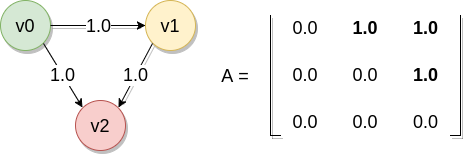
\includegraphics[width=0.5\textwidth]{figures/sample_graph}
\caption{Sample Graph Representation}
\label{fig:sample_graph}
\end{figure}

\begin{figure}[ htbp ] 
\begin{equation}
\#Edges = A^{T} \times Identity
\end{equation}
\begin{equation}
\#Edges = 
\left(\begin{array}{ccc} 0 & 0 & 0 \\ 1 & 0 & 0 \\ 1 & 1 & 0 \end{array}\right) \times
\left(\begin{array}{c} 1 \\ 1 \\ 1 \end{array}\right) 
= \left(\begin{array}{c} 0 \\ 1 \\ 2 \end{array}\right) 
\end{equation}
\caption{Incoming Edges Algorithm}
\label{fig:sample_algorithm}
\end{figure} 

\begin{lstlisting}[emph={Assign, Process, Apply}, emphstyle=\color{blue}, numbers=none, escapechar=\%, language=Python, caption=Graph Vertex Processing Model]
GraphProgram(%\textit{G}%, %\textit{P}%, %\textit{N}%) :
  for %\textit{N}% iterations :
    x := Assign(%\textit{P}%)
  	y := Process(%\textit{G}%,x)
  	%\textit{P}% := Apply(%\textit{P}%,y)	  
  
e.g. FindIncomingEdges(%\textit{G}%=A, %\textit{P}%=%\textit{\textbf{I}}%, %\textit{N}%=1) :
       Assign(%\textit{P}%)    := %\textit{P}%
  with Process(%\textit{G}%,x) := %\textit{G}% * x
       Apply(%\textit{P}%,y)   := y
\end{lstlisting}

A large variety of programming models have been proposed for describing Graph algorithms, expressing computation using vertex operations on matrices \cite{GraphMat} \cite{GraphLab}, \cite{Pregel}, \cite{MapGraph} \cite{GraphX} task-based models \cite{Galois} or domain-specific languages \cite{GreenMarl}. The vertex programming model has show great adoption for its ease of abstraction for describing algorithms using Linear Algebra and its efficient computation on commodity multi-core processors.

Figure \ref{fig:sample_graph} shows a simple 3 vertices graph example with its corresponding 3x3 matrix representation. For every edge between a source and destination vertex, the corresponding row and column entry in the matrix is activate. For instance, the matrix entry in row 0 and column 1 represents the edge between source \textit{v0} and destination \textit{v1}. using the matrix representation, we can apply an algorithm on the graph to calculate the total number of incoming edges at each vertex. This algorithm can be expressed using a simple matrix-vector operation as shown in equations (1) and (2) in Figure \ref{fig:sample_algorithm}. Several graph algorithms, including Breadth First Search (BFS) \cite{BFS}, PageRank \cite{PageRank}, Single Source Shortest-Path (SSSP) \cite{SSSP}, can be described similarly using the vertex programming model \cite{GraphMat}.

Listing 1 shows the three stages of a generalized graph vertex processing model - \textit{Assign}, \textit{Process} and \textit{Apply}, given a graph \textit{G}, some vertex properties \textit{P} and an iteration count \textit{N}. The \textit{Assign} stage generates an input vector \textit{x} using the vertex properties \textit{P}. The \textit{Process} stage applies the input vector \textit{x} to the graph \textit{G} and generates an output vector \textit{y}. The\textit{ Apply} gather the resulting output vector to update the vertex properties for the next iteration. The graph program executes the three stages for several iterations until it converges. A direct mapping of our incoming edges algorithm to this processing model is also provided in Listing 1, where the identity vector is used for the vector properties. The \textit{Assign} and \textit{Apply} stages of this program are simple identity operators, while the \textit{Process} stage perform a matrix-vector multiplication. The input graph can be represented as a sparse matrix and the computation done using a Sparse Matrix-Sparse Vector Multiplication (SpMSpV) kernel which can be accelerated on multi-core CPUs \cite{GraphMat} or on GPUs \cite{MapGraph}. FlexGraph's objective is to provide a more energy efficient graph processing backend using a FPGA for hardware acceleration \cite{Catapult}.

\subsection{Intel Heterogeneous CPU-FPGA Platform}

\begin{figure}[htbp]
\centering
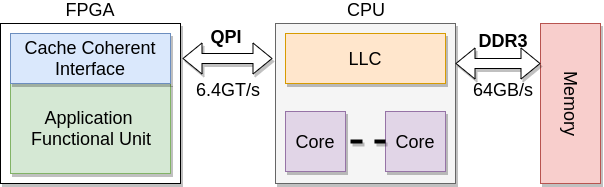
\includegraphics[width=0.5\textwidth]{figures/harp_arch}
\caption{Intel HARP Architecture}
\label{fig:harp_arch}
\end{figure}

With the rising adoption of FPGAs in production data centers \cite{Catapult}, there is a need to increase its ecosystem by making them more energy efficient and accessible to both the users and designers. Modern CPU-FPGA platforms \cite{CPU-FPGA} provide tightly-coupled shared-memory CPU-FPGA integration \cite{CAPI} \cite{CCI}, making then easier to program and providing and efficient for collaborative execution.  

\subsection{Collaborative CPU-FPGA Computation}

\section{FlexGraph Architecture}

In this section, we describes the overall architecture of the FlexGraph Accelerator.

\subsection{The DCSC Matrix Format}

\begin{figure}[htbp]
\centering
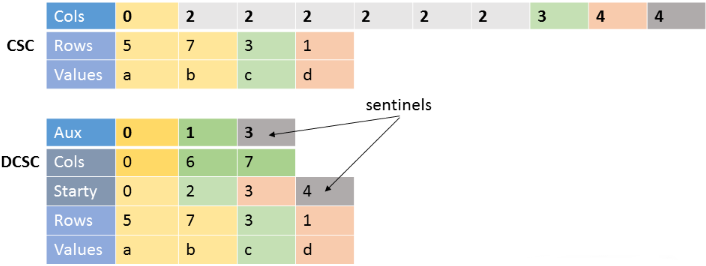
\includegraphics[width=0.4\textwidth]{figures/DCSC_matrix_format}
\caption{DCSC hyperspace matrix format}
\label{fig:DCSC_matrix_format}
\end{figure}

Most Data Analytics graphs are represented in a sparse matrix format to save memory space due to the large amount of empty edges that exist. FlexGraph's matrices are stored using a Doubly Compressed Sparse Column (DCSC) \cite{DCSC} format. The format allows minimal traversal into the sparse matrix structure, saving necessary memory bandwidth when fetching empty columns. Figure \ref{fig:DCSC_matrix_format} shows a sample matrix A = \{(0,5,a), (0,7,b), (6,3,c), (7,1,d)\} with four non-zero edges (src, dst, weight) encoded using DCSC versus the conventional CSC \cite{CSC} format. The traversal over CSC requires accessing all consecutive column ranges \textit{(cols[i+2] - cols[i])} even though most of the distances are empty. DCSC saves on bandwidth by using an additional indirection  buffer inside its structure to only encode non-zero columns. It is important to note that the saving this format introduced additional space and compute overhead that only pays off when the matrix is very large and sparse, a prevalent characteristic of Graph Analytics datasets.

\subsection{The Sparse Matrix Multiplication Kernel}

FlexGraph architecture implements a custom Sparse Matrix Vertex Multiplication (SPMV) kernel. Its architecture diverges from conventional implementations in two ways: First, it uses the dirty masks from  the input vertices to select the edges to process and return a new dirty masks capturing the intersection of the active input vertices and the non-zero edges actually visited. Second, it matrix data structure (DCSC) contains an additional indirection buffer for accessing the matrix columns. These two properties present unique performance challenges when designing the accelerator. Listing 1 shows the pseudo-code of the SPMV kernel. The program iterates through each column and fetch the corresponding input vertex active mask to check if the column should be process, then access all the non-zero rows of the matrix for that column to evaluate each edge. In the code's comments on the right are highlighted the different types performance hogs present; semi-random memory accesses (*), fully-random memory accesses (!) and control branches (?). The memory accesses for the columns and rows data (lines 4 and 9) are semi-random because only the access cannot be predicted and after that the address is simply incremented. FlexGraph's architecture attempts to address some of those performance hogs using several optimizations detailed in section 4.

\begin{lstlisting}[language=Python, caption=Pseudo-code for SPMV kernel]
def SPMV_kernel(x_values, x_activemask) :
  y_values = {0}, y_activemask = {0}
    for col in (c_start, c_end) :            	
      (a_x, r_start, r_end) = coldata[col]   # *
      x_value  = x_values[a_x]               # !
      x_active = x_activemask[a_x]           # !
      if (x_active):                         # ?
        for row in (r_start, r_end):         
          (a_y, a_value) = rowdata[row]      # *
          y_values[a_y] += a_value * x_value # !
          x_activemask[a_y] = true           # !
  return (y_values, y_activemask)
\end{lstlisting}

\subsection{FlexGraph Microarchitecture}

Externally, FlexGraph input and output signals implement an Accelerator Functional Unit (AFU) interface defined by Intel's Accelerator Abstraction Layer (AAL) \cite{Intel-FPGA}. AFUs implementing the interface are able to bind with the FPGA's board support package (BSP) and seamlessly communicate with the AAL software runnign on the host processor. Listing 2 shows AAL device interface implementation using Cocoh's API. Our FlexGraph Accelerator's class in Cocoh simply derives from this interface and override the \textit{initialize()} function to provide its implementation and Cocoh takes care of generating the corresponding verilog module. It implements three input signals \textit{(start, qpi\_in, ctx)} and two output signals \textit{(qpi\_out, done)}. The AFU starts execution when the \textit{start} signal is asserted and communicate completion by asserting the \textit{done} signal. The \textit{ctx} signal provides application's specific data like constants and buffers address in the case of FlexGraph. The \textit{qpi} in/out signals implement Intel Quick Path Interconnect (QPI) interface \cite{QPI}, providing single channel read/write ports for accessing external shared memory. The FPGA socket hosts a 64-byte cache coherent interface (CCI) \cite{CCI} that connects to the host processor's last level cache (LLC) via QPI.     

\begin{lstlisting}[language=C++, caption=AAL Device Interface in Cocoh C++]
class aal_device {
public: 
  virtual out_t initialize()(
    const ch_logic& start, 
    const qpi::in_t& qpi_in, 
    const afu_ctx_t& ctx, 
    qpi::out_t& qpi_out, 
    ch_logic& done
  ) const = 0;  
};
\end{lstlisting}

\begin{figure}[htbp]
\centering
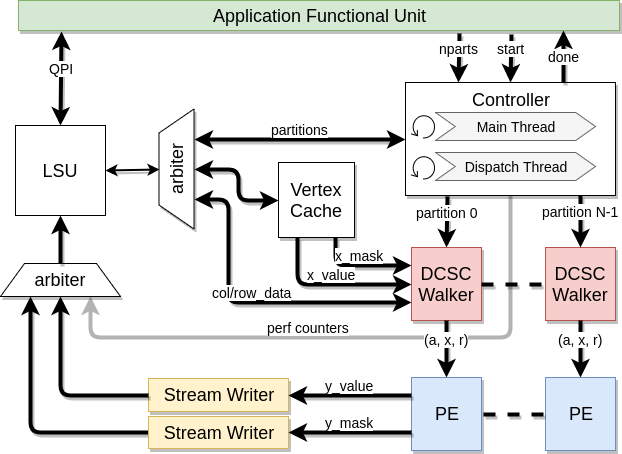
\includegraphics[width=0.4\textwidth]{figures/microarchitecture}
\caption{FlexGraph Microarchitecture}
\label{fig:microarchitecture}
\end{figure}

Figure \ref{fig:microarchitecture} illustrates FlexGraph accelerator microarchitecture. It is comprised of four main module types, a controller, processing elements (PEs), a load store unit (LSU) and vertex caches. The main controller is responsible for starting the accelerator, scheduling tasks for execution, reporting hardware counters and terminating the execution. The processing elements execute partition tasks assigned to them by the controller and communicate with the LSU to access the matrix and vertex data for their partition. They are also responsible for sending their final output result back to memory. The LSU is the module responsible for managing external communication between the accelerator and memory via the QPI interface. It directly binds to the QPI ports defined in listing 2.
The vertex caches store intermediate vertex data and active masks for sharing between the processing elements. FlexGraph processing pipeline sightly resembles the SPMV execution steps illustrated in listing 1. We made several important modifications to it to improve performance.  

\section{FlexGraph Parallelization}

The first optimization we performed in FlexGraph early during the design phase was the support of multiple processing units. The reasoning behind it was to extract the maximum bandwidth out of the LSU such that the QPi is always busy processing a request when some processing element are stalled waiting for their data to return. the other advantage of parallelization for FlexGraph is to increase the overall accelerator throughput by processing multiple a larger chunk of the workload per unit of time. The scheduling of the partitions for execution on the processing elements is controlled by a dispatch unit inside the main controller module. The dispatch unit fetches partitions data from the LSU and pass down each partition in a first come first serve fashion to the processing elements.

\subsection{DCSC Matrix partitioning}

\begin{figure}[htbp]
\centering
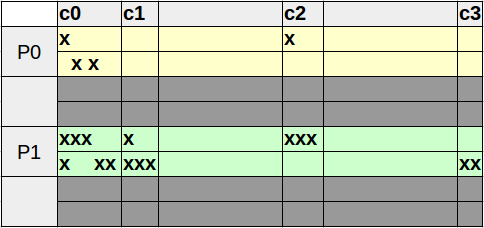
\includegraphics[width=0.4\textwidth]{figures/matrix_partitioning}
\caption{DCSC Matrix Partitioning}
\label{fig:matrix_partitioning}
\end{figure}

To enable the parallelization of FlexGraph tasks, the DCSC sparse matrix is first partitioned into aligned partitions of 32 consecutive rows containing non-zero edges. we choose a partition size of 32 mainly to match the 32-bit size of the bitmasks encoding the vertices that are active. These masks are used by the software on the host processor to determine the regions of the acceleration's output buffer that have been updated. Figure \ref{fig:matrix_partitioning} illustrates sample matrix partitioning in which the non-zero horizontal regions have been broken into two partitions P0 and P1. The non-zero column ranges \textit{(c0, c1, c2, c3)} represent the selected chunks covered by each partition. Partition P0 will only contain ranges \textit{c0} and \textit{c2} while P2 has non-zeros in all four ranges. The partitioning scheme is not ideal because of the workload in-balance that might exist when the number of non-zero varies disproportionally between partitions.  

\subsection{Synchronising Memory Accesses}

\begin{figure}[htbp]
\centering
\includegraphics[width=0.35\textwidth]{figures/write_masks_synchronization}
\caption{Active Masks Write Synchronization}
\label{fig:write_masks_synchronization}
\end{figure}

An implementation challenge we faced when supporting multiple processing elements in FlexGraph was the synchronization of write accesses for the output active masks. Because the LSU data transfer granularity is 64 byte (matching CCI \cite{CCI}), FlexGraph need to manage shared write accesses to the same block to avoid having a processing element override the content of another one. Luckily this doesn't pose any problem for writing out partition output values because the 32 rows within a partition occupy 32 * 4 bytes = 2 x 64 bytes blocks. Because the partitioning reinforces 32 rows alignment, each processing element can safely write into their assigned blocks. However, writing out the active masks poses a challenge because a single 4-byte mask encodes the active states of all 32 rows in a partition. This causes the processing elements to potentially share a single 64-byte block when writing the masks out to memory. To alleviate the contention, FlexGraph keep N active 64-byte blocks locally assigned to either one of the N processing elements. It assigns an ownership bit mask to each block to track their reference count and the processing element assigned to them. It also tracks the current address value assigned to each block. When a processing element is ready to write its 4-byte active mask, it passes the mask address and value to the LSU. The LSU goes to last active block the processing element previous wrote to and check if the block address matches. If so, it simply adds the new content to the existing block. If there is no match, it clears its ownership bit and flushes the block to memory if the ownership mask goes to zero. Then it looks up the other active block if anyone already has the address to use it, otherwise if it acquires the last unused block. Figure \ref{fig:write_masks_synchronization} shows a simplified illustration of the scheme with two processing elements. We don't need to keep more than N blocks in local storage for this scheme to work because the block address references are always incremental and never regress, meaning that there is always going to be free block available to use. It is important to also point out that for this scheme to work, the operation has to be atomic. FlexGraph has a single communication channel between all processing elements and the LSU which does some round robin arbitration and blocks the write mask request until it is committed. We also investigated an alternative solution to avoid this synchronization, which is simply increasing the partition size to 16 * 32 rows, allowing the aggregated active masks to occupy a full 64-byte block. They were two major issues with this approach. Firstly, the total size of all resident partitions will be too large if we support multiple processing elements. Secondly, it will worsen the workload imbalance that is already present with 32 rows.     

\section{FlexGraph Optimizations}

This section describes some optimizations we added to FlexGraph to improve its performance. 

\subsection{Optimizing Memory Accesses via Stream Buffers}

\begin{figure}[htbp]
\centering
\includegraphics[width=0.4\textwidth]{figures/stream_buffers}
\caption{Stream Buffers}
\label{fig:stream_buffers}
\end{figure}

As stated before, FlexGraph's LSU transfer granularity is 64 bytes, which is much larger than the 4 bytes of elements accessed by the processing elements. To save on bandwidth, the LSU uses stream buffers that fetch a 64-byte blocks of data but extracts 4-byte elements at the time. It is implemented using a fifo structure in the back-end where 64-byte responses from QPI go
 into. In the front-end, there is a temporary 64-byte block that is extracted from the fifo on demand to deliver 4-byte element at the time. We employ a shift register to extract the 4-byte element to pass it to the processing element. Figure \ref{fig:stream_buffers} shows an illustration of the stream buffer concept.
   
\subsection{Caching Vertex Values and Masks}

Another optimization we implemented in FlexGraph is the caching of vertex values and masks. Looking at the SPMV speudo-code in listing 1, we can observe in lines 5 and 6 that there is a random memory access to buffers \textit{x\_values} and \textit{x\_activemask}. FlexGraph employs a stream buffer like concept to consume 64-byte vertex data once they arrive inside the processing element to each iteration loop. However, the same block can be referenced by another processing element and sharing them inside the cache structure can save unnecessary memory traffic. We implemented two small fully associative caches with first-in-First-out replacement to hold active vertex data during execution. The caches are implemented inside the LSU which is responsible for managing them. When a vertex request arrives from a processing element, the LSU first looks up the cache if the block is already present and return it. If the block is not there, it sends the request to QPI. QPI output interface support a 14-bit metadata field that is used to identify the block once it is returned. We use that field to store the index of the block such that we can compute the cache tag when it arrives. Because the cache is small, we implemented a one cycle tag lookup for the LSU to known if the block is present and accessible.

\subsection{Executing Non-blocking Memory writes}

FlexGraph memory writes are all non-blocking, this applies to both the output values and active masks. This allows the processing elements to push their write request and resume execution while the LSU is processing them. Upon write responses from the QPI channel, the LSU internally keeps track of the count of outstanding requested to ensure that all writes have completed. The QPI interface exposes two write response ports by which the memory replies could be sent. This allows servicing two responses simultaneously. The LSU implements a mechanism to process both channels simultaneously when they are active. At completion time when all processing elements are done executing the current run, the controller waits for all outstanding write requests to complete before asserting the \textit{done} signal.

\section{FlexGraph Software-Hardware Codesign}
\section{Experimental Setup}

\subsection{Cocoh's Simulation}

\subsection{Intel AAL Interface}

\subsection{Intel QPI Emulation}

\subsection{Graph Datasets}

\section{Results Analysis}

\subsection{Overall Performance}

\subsection{The Impact of Parallelism}

\subsection{The Impact of Memory Optimizations}

\subsection{FlexGraph Performance Hogs}

\subsection{Hardware Cost Evaluation}
\section{Related Work}

\subsection{Graphicionado}

\subsection{GraphOps}

\subsection{Tesseract}
\section{Future Work}

\subsection{Performance Optimization}
* Prefetching xindices and ystarts blocks
* Increasing the number of processing cores
* LSU active PEs mask optimization
* write mask synchronization issue

\subsection{FPGA Evaluation}

\subsection{Energy and Power Evaluation}
\section{Conclusion}
\section{Acknowledgment}

The authors gratefully acknowledge the insightful feedback and input from Professor Heysoon Kim from Georgia Institute of Technology and David Sheffield from Intel Labs.\\
\\
This research was supported by a grant from the National Science Foundation under grant CCF-1533767.

% Can use something like this to put references on a page
% by themselves when using endfloat and the captionsoff option.
\ifCLASSOPTIONcaptionsoff
  \newpage
\fi

\begin{small}
\bibliography{reference}
\bibliographystyle{abbrv}
\end{small}

% that's all folks
\end{document}